% Generated by scripts/08_build_latex.py from report/report_template.tex.
% Self-contained: compile with pdflatex (run twice for references) or upload to Overleaf.
\documentclass[10pt,a4paper]{article}

\usepackage[utf8]{inputenc}
\usepackage[T1]{fontenc}
\usepackage{lmodern}
\usepackage[margin=1.8cm]{geometry}
\usepackage{amsmath,amssymb}
\usepackage{graphicx}
\usepackage{booktabs}
\usepackage{multirow}
\usepackage{caption}
\usepackage{subcaption}
\usepackage[compact]{titlesec}
\usepackage{enumitem}
\usepackage{xcolor}
\usepackage{microtype}
\usepackage[colorlinks=true,linkcolor=blue!50!black,citecolor=blue!50!black,urlcolor=blue!50!black]{hyperref}

\captionsetup{font=small,labelfont=bf,skip=3pt}
\captionsetup[sub]{font=small,skip=1pt}
\setlist{itemsep=1pt,topsep=2pt,parsep=0pt,leftmargin=*}
\setlength{\textfloatsep}{8pt plus 2pt minus 2pt}
\setlength{\floatsep}{6pt plus 2pt minus 2pt}
\setlength{\intextsep}{6pt plus 2pt minus 2pt}
\setlength{\abovedisplayskip}{4pt}
\setlength{\belowdisplayskip}{4pt}
\setlength{\parskip}{2pt}
\renewcommand{\arraystretch}{1.05}

\newcommand{\studentname}{Jagini Mohit}
\newcommand{\rollno}{IMT2023528}
\newcommand{\HLS}{\mathbf{h}_{\mathrm{LS}}}

\title{\vspace{-1.2cm}\textbf{ChannelNet: Deep-Learning-Based OFDM Channel Estimation\\as Image Super-Resolution and Restoration}}
\author{COM 837 -- Machine Learning for Wireless Communication -- Assignment 3\\
Name: \studentname \qquad Roll No.: \rollno \qquad 23-11-2026}
\date{\vspace{-0.9cm}}

\begin{document}
\maketitle

% ----------------------------------------------------------------------------
\section{Objective}

The time--frequency response of a SISO-OFDM channel over one LTE sub-frame ($72$ sub-carriers $\times$ $14$
OFDM symbols) is treated as a 2-D image of which only a few noisy pilot samples are observed. Following
Soltani \emph{et al.}, it is reconstructed by \textbf{ChannelNet}: an image super-resolution
network (SRCNN) followed by a denoising network (DnCNN), and compared with LS + 2-D
interpolation and the MMSE-type baselines of the paper (ideal MMSE, estimated MMSE, ideal
ALMMSE) on the VehA and SUI5 channels, for 0--30~dB SNR and 8--48 pilots per frame.

% ----------------------------------------------------------------------------
\section{System model and data generation (Task 1)}

\paragraph{OFDM grid.} LTE 1.4~MHz numerology: 72 used sub-carriers (DC excluded), 15~kHz spacing, normal
CP, 14 OFDM symbols per 1~ms sub-frame. Per resource element (eqs.~(1)--(2) of the paper)
\begin{equation}
  Y[k,l] = H[k,l]\,X[k,l] + Z[k,l],\quad Z\sim\mathcal{CN}(0,\sigma^2),\quad
  \mathrm{SNR}=\frac{\mathbb{E}|X|^2\,\mathbb{E}|H|^2}{\sigma^2}=\frac{1}{\sigma^2},\qquad
  \hat H_{\mathrm{LS}}[k_p,l_p] = \frac{Y[k_p,l_p]}{X[k_p,l_p]} .
\end{equation}
The per-sub-carrier model was verified against a full time-domain OFDM link (IFFT, CP, multipath
convolution, FFT) in \texttt{tests/test\_sanity.py}.

\paragraph{Channel models.} Both are WSSUS tapped-delay lines,
$H[k,l] = \sum_{p} \sqrt{P_p}\, g_p(t_l)\, e^{-j2\pi f_k \tau_p}$, with independent unit-power Rayleigh
processes $g_p(t)$ with a Jakes Doppler spectrum. As in the paper: 2.1~GHz carrier and 50~km/h
($f_D = 97$~Hz, coherence time 4.3~ms). \textbf{VehA} (ITU-R M.1225): 6 taps over 0--2.51~$\mu$s, RMS delay
spread 0.37~$\mu$s, coherence bandwidth 540~kHz. \textbf{SUI5}: taps at 0/4/10~$\mu$s with
0/$-5$/$-10$~dB, RMS delay spread 2.84~$\mu$s, coherence bandwidth 70~kHz (only $\approx$5 sub-carriers;
the 10~$\mu$s excess delay also exceeds the 4.7~$\mu$s CP), i.e.\ far more frequency-selective.

\paragraph{Simulator.} The paper used the Vienna LTE-A simulator. The course provided the
\textbf{Vienna 5G Link-Level Simulator}; \texttt{matlab/generate\_vienna\_channels.m} uses its
\texttt{Channel.FastFading} class (15.36~MHz sampling, built-in VehicularA, SUI5 as user-defined PDP,
\texttt{GetTransferFunction} at every OFDM-symbol centre) to generate 40\,000 frames per model. The networks
were trained on Kaggle with the project's Python implementation of the \emph{same} models
(\texttt{src/channel\_models.py}, sum-of-sinusoids Jakes fading), whose statistics match the Vienna
channels (frequency correlation at 6 sub-carriers 0.972/0.973 for VehA, 0.650/0.653 for SUI5; time
correlation across the sub-frame 0.92 for both). Section~\ref{sec:vienna} tests the trained networks on the
Vienna channels directly.

\paragraph{Pilots and data set.} Lattice pilots (Fig.~\ref{fig:pilots}): the main pattern has
\textbf{48 pilots} on OFDM symbols $\{0,4,7,11\}$, every 6th sub-carrier with alternating offset 3 (the LTE
CRS diamond). Further densities: 36 (spacing 8, baselines only), 24 (symbols $\{3,10\}$, spacing 6), 16
(spacing 9) and 8 (spacing 18); unit-energy QPSK. 40\,000 frames per channel are split
32\,000/4\,000/4\,000 (train/validation/test) as in the paper. The noise of each (split, pattern, SNR)
is drawn from a seed derived from the master seed, so all methods see the \emph{same} noisy observations.
Each complex grid becomes \textbf{two 2-D images} (real and imaginary part, Fig.~\ref{fig:gt}), normalised
by the training standard deviation 0.707.

\begin{figure}[!htbp]
  \centering
  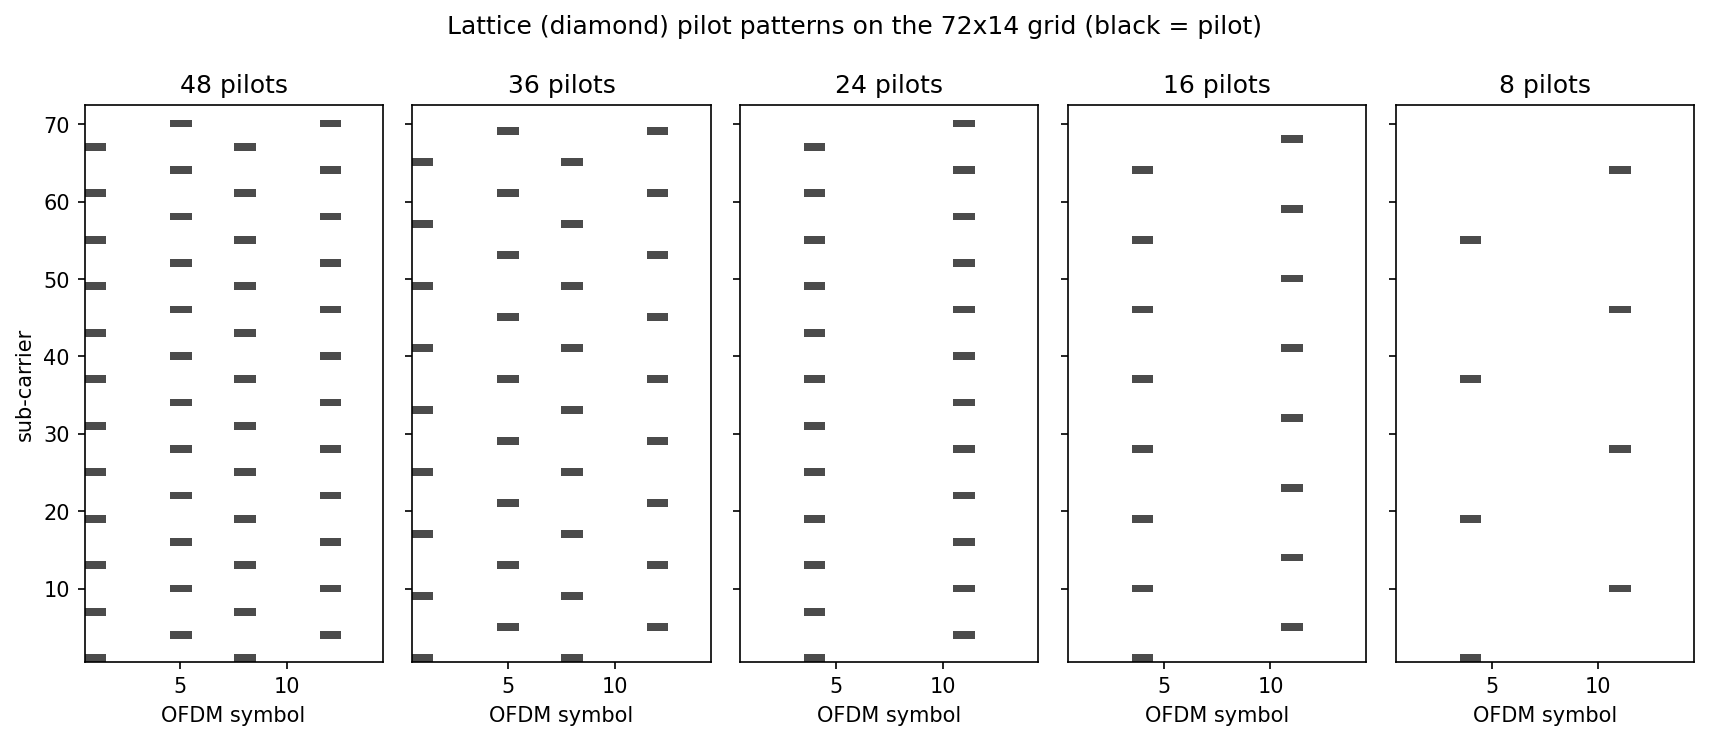
\includegraphics[width=0.66\textwidth]{Images/pilot_patterns.png}
  \caption{Lattice pilot patterns (black = pilot).}
  \label{fig:pilots}
\end{figure}

\begin{figure}[!htbp]
  \centering
  \begin{subfigure}[t]{0.42\textwidth}
    \centering
    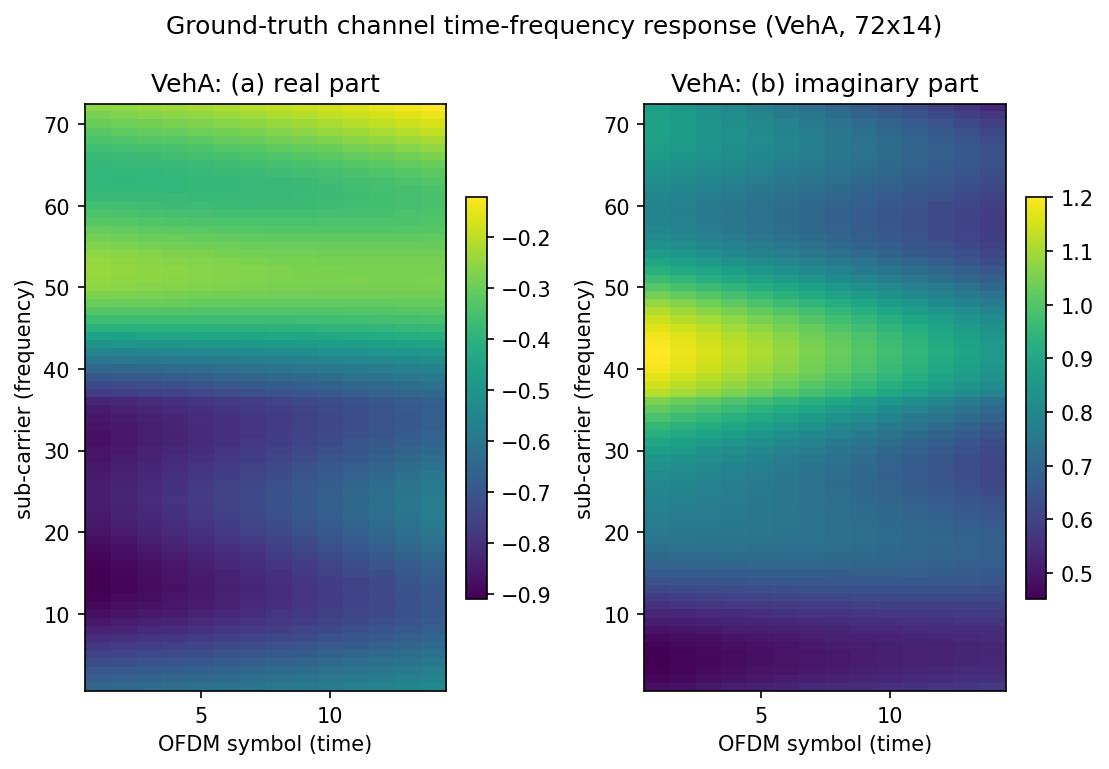
\includegraphics[width=\linewidth]{Images/fig2_ground_truth_VehA.png}
    \caption{VehA: smooth in time and frequency.}
  \end{subfigure}\hspace{0.04\textwidth}
  \begin{subfigure}[t]{0.42\textwidth}
    \centering
    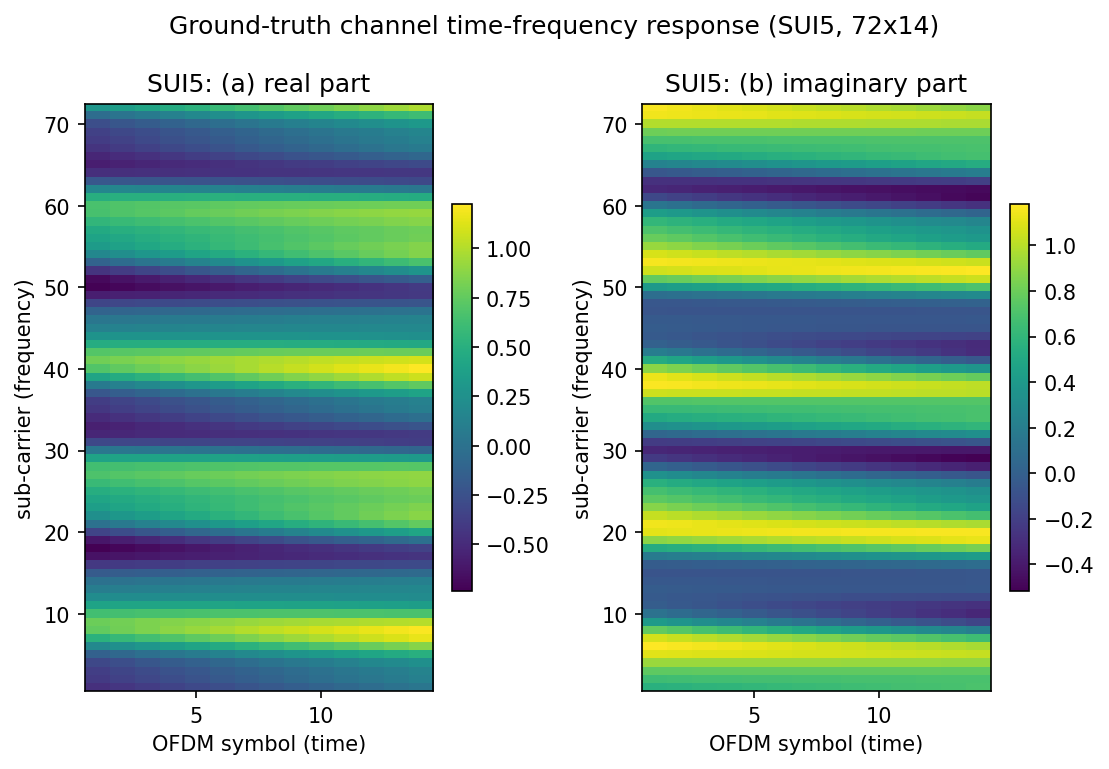
\includegraphics[width=\linewidth]{Images/fig2_ground_truth_SUI5.png}
    \caption{SUI5: fast ripples across frequency.}
  \end{subfigure}
  \caption{Ground-truth real and imaginary channel images (cf.\ Fig.~1 of the paper).}
  \label{fig:gt}
\end{figure}

% ----------------------------------------------------------------------------
\section{Conventional channel estimation (Task 2)}

With fixed pilot positions every conventional estimator is linear, $\hat{\mathbf h} = \mathbf W\HLS$,
$\mathbf W\in\mathbb C^{1008\times P}$.
\begin{itemize}
  \item \textbf{LS + 2-D interpolation}: linear (Delaunay), cubic and Gaussian-RBF (as in the reference code
    of the paper) interpolation over the (sub-carrier, symbol) plane.
  \item \textbf{Ideal MMSE} (eq.~(5) of the paper): $\hat{\mathbf h} = \mathbf R_{hp}(\mathbf R_{pp} +
    \sigma^2\mathbf I)^{-1}\HLS$ with the exact $1008\times1008$ covariance of the 32\,000 true training
    channels -- the genie lower bound.
  \item \textbf{Estimated MMSE}: same filter, covariance estimated from 2\,000 received (noisy LS +
    linearly interpolated) frames at the operating SNR, minus the known noise term
    $\sigma^2\mathbf W_{\mathrm{int}}\mathbf W_{\mathrm{int}}^H$.
  \item \textbf{Ideal ALMMSE} (\v{S}imko \emph{et al.}, course material): assumes
    $\mathbf R_h = \mathbf R_{\mathrm{time}}\otimes\mathbf R_{\mathrm{freq}}$ and filters the interpolated
    LS grid separately in frequency and time, $\hat{\mathbf H} = \mathbf B_{\mathrm{freq}}\hat{\mathbf
    H}_{\mathrm{LS}}\mathbf C_{\mathrm{time}}^T$, with the rank-one filters of eqs.~(12)--(19) of \v{S}imko \emph{et al.}
    ($N_{\mathrm{freq}}=5$, $N_{\mathrm{time}}=2$ eigenvalues).
\end{itemize}

% ----------------------------------------------------------------------------
\section{ChannelNet (Tasks 3 and 4)}

The LS pilot values are interpolated onto the $72\times14$ grid (Gaussian RBF, as in the paper) to form the
low-resolution image; the SRCNN maps it to the full-resolution channel and the cascaded DnCNN removes the
remaining noise by residual learning: $\hat{\mathbf H} = f_{\mathrm{IR}}(f_{\mathrm{SR}}(\mathrm{interp}
(\hat{\mathbf H}_{\mathrm{LS}})))$. Real and imaginary parts are separate single-channel images and all
convolutions use `same' padding (Table~\ref{tab:arch}; 8\,129 and 0.67\,M parameters).

\begin{table}[!htbp]
  \centering
  \caption{ChannelNet architecture (as in the paper).}
  \label{tab:arch}
  \small
  \begin{tabular}{llccl}
    \toprule
    stage & layer & kernel & filters & activation \\
    \midrule
    SR (SRCNN) & conv 1 / 2 / 3 & $9\times9$ / $1\times1$ / $5\times5$ & 64 / 32 / 1 & ReLU / ReLU / linear \\
    \midrule
    \multirow{3}{*}{IR (DnCNN, 20 layers)} & conv 1 & $3\times3$ & 64 & ReLU \\
     & conv 2--19 & $3\times3$ & 64 & BN + ReLU \\
     & conv 20 & $3\times3$ & 1 & residual: $\hat{\mathbf x} = \mathbf y - \mathcal R(\mathbf y)$ \\
    \bottomrule
  \end{tabular}
\end{table}

% ----------------------------------------------------------------------------
\section{Training procedure and reproducibility (Task 5)}

\begin{itemize}
  \item \textbf{Two-stage training} (eqs.~(7)--(8) of the paper): the SRCNN is trained first, then frozen
    while the DnCNN is trained on its outputs,
    $C_1 = \frac{1}{|\mathcal T|}\sum_{i}\|f_{\mathrm{SR}}(\mathbf X_i^{\mathrm{LR}}) - \mathbf H_i\|_F^2$,
    $C_2 = \frac{1}{|\mathcal T|}\sum_{i}\|f_{\mathrm{IR}}(f_{\mathrm{SR}}(\mathbf X_i^{\mathrm{LR}})) -
    \mathbf H_i\|_F^2$. Adam, learning rate $10^{-3}$, batch 128 (as in the paper); ReduceLROnPlateau
    (factor 0.5) and early stopping on the validation loss, keeping the best weights; at most 150 (SR) /
    40 (IR) epochs.
  \item \textbf{SNR-specific training} as in the paper: ``deep low-SNR'' networks at \textbf{12~dB} and
    ``deep high-SNR'' networks at \textbf{22~dB}, both tested over 0--30~dB. The pilot study uses 22~dB
    networks for 48/24/16/8 pilots. A \emph{multi-SNR} network (SNR $\sim\mathcal U[0,30]$~dB per frame)
    tests one remedy for the SNR problem (Section~\ref{sec:discussion}). In total 14 ChannelNets were trained.
  \item \textbf{Cost and convergence}: Kaggle Tesla T4, PyTorch with fp16 mixed precision, 23--33~min per
    model, 424~min in total. The SR stage mostly reached the 150-epoch limit while still improving slowly;
    the DnCNN converged in 17--40 epochs. Training and validation losses stay close (Fig.~\ref{fig:loss}),
    so there is no overfitting (64\,000 training images), and the IR stage clearly lowers the loss.
  \item \textbf{Reproducibility}: master seed 2026 from which every random stream (channels, noise, weight
    initialisation, batch order) is derived; cuDNN deterministic mode; settings in
    \texttt{configs/final.yaml}; every checkpoint stores a \texttt{meta.json} (configuration, seed,
    normalisation, environment). Regenerating the data locally reproduces the Kaggle data exactly.
\end{itemize}

\begin{figure}[!htbp]
  \centering
  \begin{subfigure}[t]{0.49\textwidth}
    \centering
    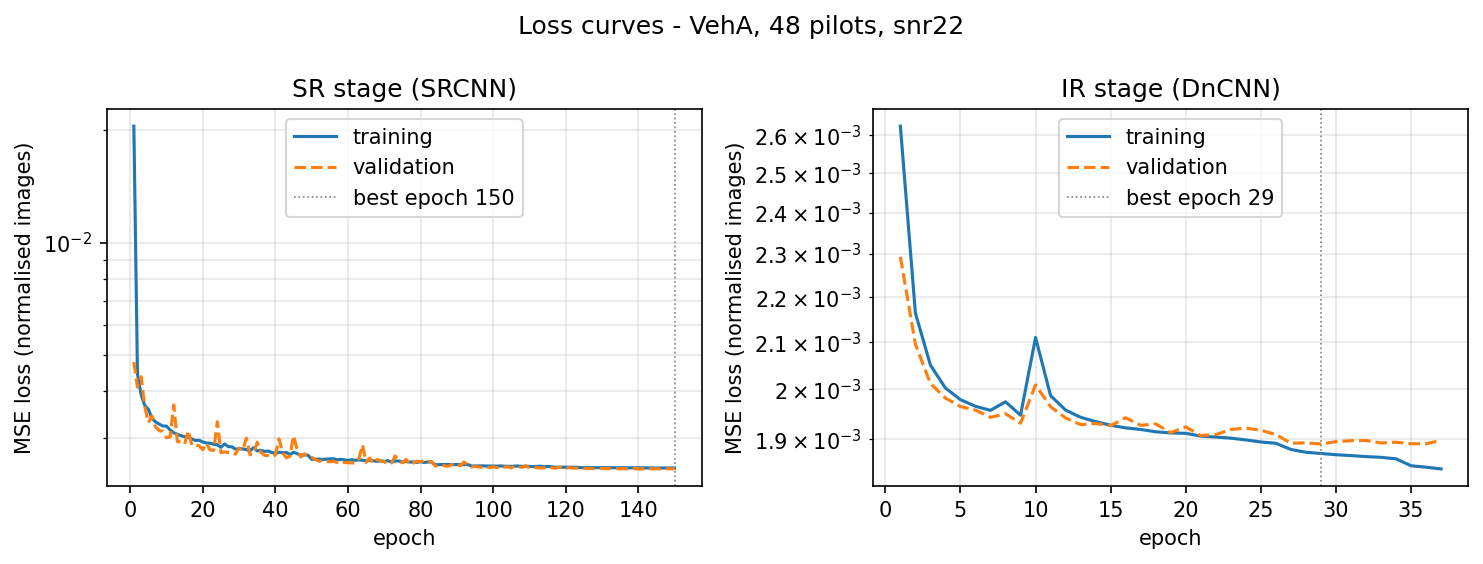
\includegraphics[width=\linewidth]{Images/loss_curves/loss_VehA_p48_snr22.png}
    \caption{VehA, 48 pilots, 22~dB.}
  \end{subfigure}\hfill
  \begin{subfigure}[t]{0.49\textwidth}
    \centering
    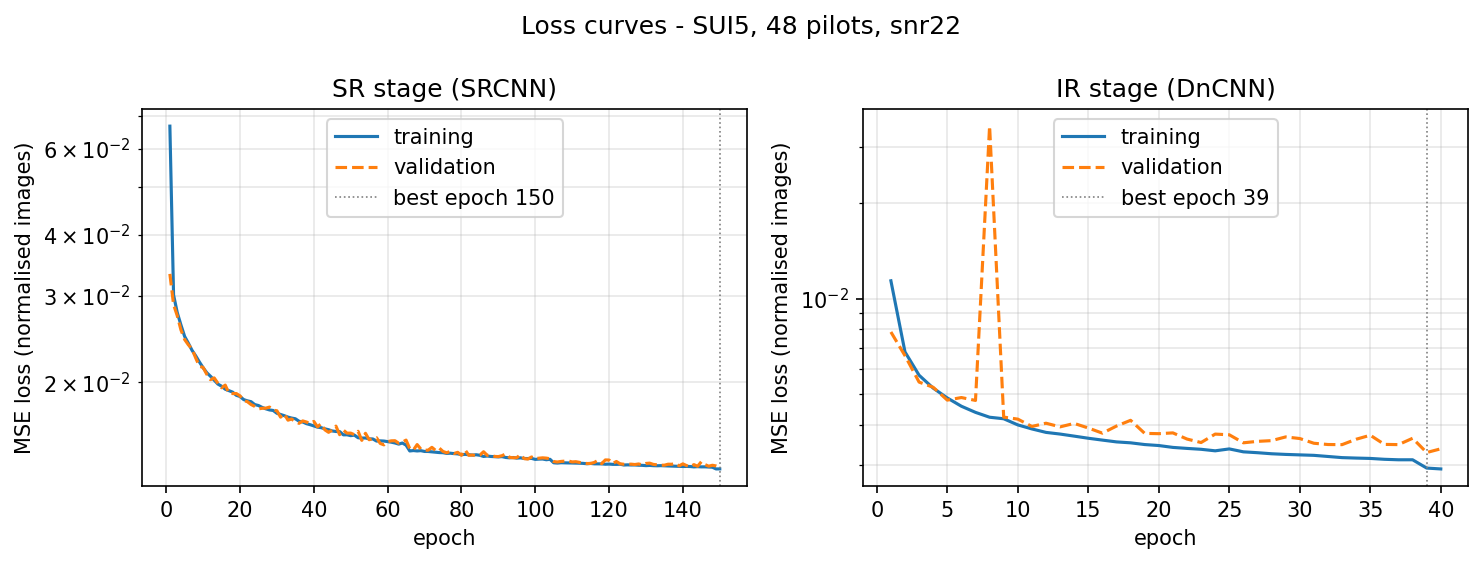
\includegraphics[width=\linewidth]{Images/loss_curves/loss_SUI5_p48_snr22.png}
    \caption{SUI5, 48 pilots, 22~dB.}
  \end{subfigure}
  \caption{Training/validation loss of the SR and IR stages (all 14 models:
    \texttt{results/figures/loss\_curves/}).}
  \label{fig:loss}
\end{figure}

% ----------------------------------------------------------------------------
\section{Results (Task 6)}

All results use the 4\,000 test frames. In the tables, LS-lin = LS + linear interpolation, SR-$s$ = SRCNN
output only, CN-$s$ = full ChannelNet trained at $s$~dB (``mix'' = multi-SNR); \textbf{bold} = best
estimator that does not use genie statistics.

\subsection{MSE versus SNR (paper Figs.~3 and 4)}

\begin{figure}[!htbp]
  \centering
  \begin{subfigure}[t]{0.49\textwidth}
    \centering
    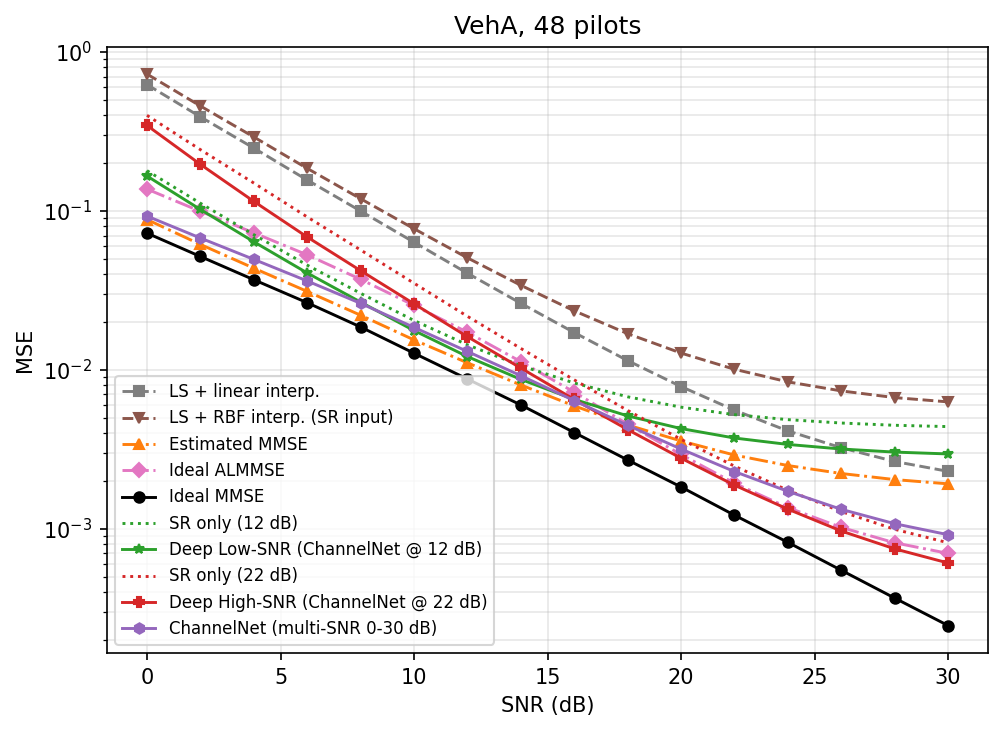
\includegraphics[width=\linewidth]{Images/fig3_VehA_mse_vs_snr.png}
    \caption{VehA (paper Fig.~3).}
  \end{subfigure}\hfill
  \begin{subfigure}[t]{0.49\textwidth}
    \centering
    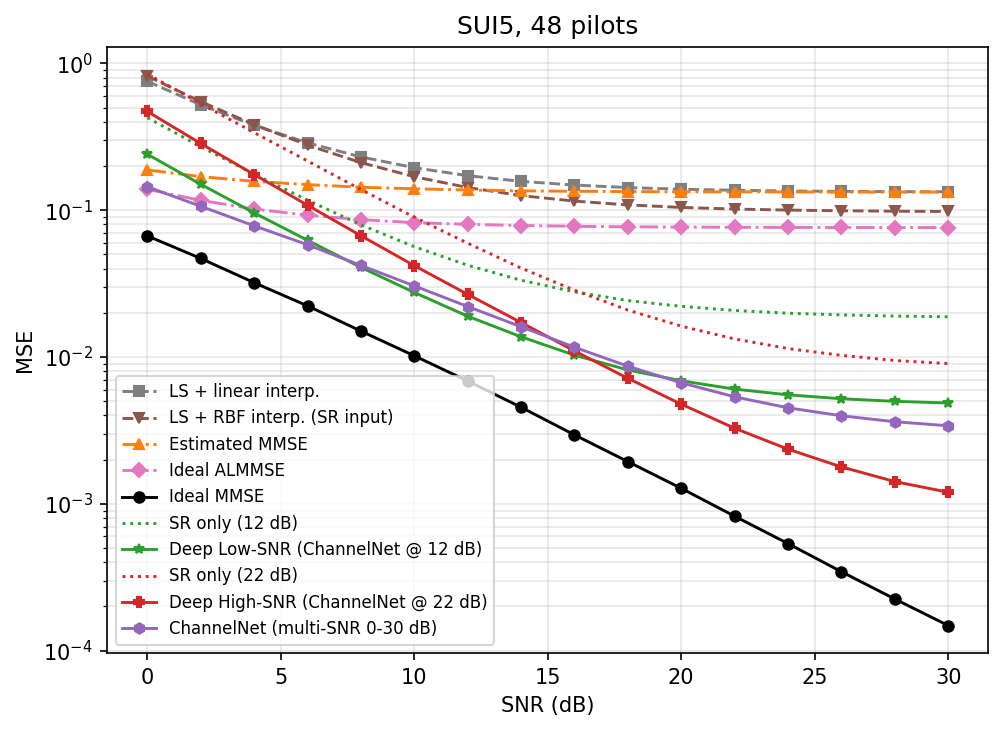
\includegraphics[width=\linewidth]{Images/fig4_SUI5_mse_vs_snr.png}
    \caption{SUI5 (paper Fig.~4).}
  \end{subfigure}
  \caption{MSE vs.\ SNR, 48 pilots.}
  \label{fig:mse_snr}
\end{figure}

\begin{table}[!htbp]
  \centering
  \caption{MSE vs.\ SNR, 48 pilots (selected SNRs).}
  \label{tab:mse_snr}
  \small
  \setlength{\tabcolsep}{4.5pt}
  \begin{tabular}{rcccccccc}
    \toprule
    SNR (dB) & LS-lin & Est. MMSE & Ideal ALMMSE & Ideal MMSE & SR-22 & CN-12 & CN-22 & CN-mix \\
    \midrule
    \multicolumn{9}{l}{\textit{VehA}} \\
    0 & 6.23e-1 & \textbf{8.82e-2} & 1.37e-1 & 7.25e-2 & 3.99e-1 & 1.66e-1 & 3.45e-1 & 9.28e-2 \\
    6 & 1.56e-1 & \textbf{3.11e-2} & 5.29e-2 & 2.65e-2 & 9.16e-2 & 4.07e-2 & 6.85e-2 & 3.62e-2 \\
    12 & 4.05e-2 & \textbf{1.11e-2} & 1.72e-2 & 8.76e-3 & 2.17e-2 & 1.21e-2 & 1.62e-2 & 1.31e-2 \\
    20 & 7.85e-3 & 3.57e-3 & 2.94e-3 & 1.83e-3 & 3.66e-3 & 4.27e-3 & \textbf{2.78e-3} & 3.18e-3 \\
    22 & 5.58e-3 & 2.91e-3 & 1.94e-3 & 1.22e-3 & 2.48e-3 & 3.73e-3 & \textbf{1.88e-3} & 2.29e-3 \\
    30 & 2.30e-3 & 1.92e-3 & 7.01e-4 & 2.47e-4 & 8.18e-4 & 2.96e-3 & \textbf{6.10e-4} & 9.19e-4 \\
    \midrule
    \multicolumn{9}{l}{\textit{SUI5}} \\
    0 & 7.55e-1 & 1.88e-1 & 1.39e-1 & 6.68e-2 & 8.46e-1 & 2.40e-1 & 4.70e-1 & \textbf{1.44e-1} \\
    6 & 2.88e-1 & 1.49e-1 & 9.25e-2 & 2.23e-2 & 2.16e-1 & 6.24e-2 & 1.08e-1 & \textbf{5.82e-2} \\
    12 & 1.72e-1 & 1.37e-1 & 8.01e-2 & 6.86e-3 & 5.96e-2 & \textbf{1.90e-2} & 2.67e-2 & 2.21e-2 \\
    20 & 1.39e-1 & 1.33e-1 & 7.67e-2 & 1.27e-3 & 1.62e-2 & 6.89e-3 & \textbf{4.77e-3} & 6.67e-3 \\
    22 & 1.37e-1 & 1.33e-1 & 7.65e-2 & 8.23e-4 & 1.33e-2 & 6.04e-3 & \textbf{3.27e-3} & 5.36e-3 \\
    30 & 1.33e-1 & 1.33e-1 & 7.62e-2 & 1.48e-4 & 9.02e-3 & 4.86e-3 & \textbf{1.20e-3} & 3.40e-3 \\
    \bottomrule
  \end{tabular}
\end{table}

\subsection{Deep high-SNR case: VehA and SUI5 separately}

\begin{figure}[!htbp]
  \centering
  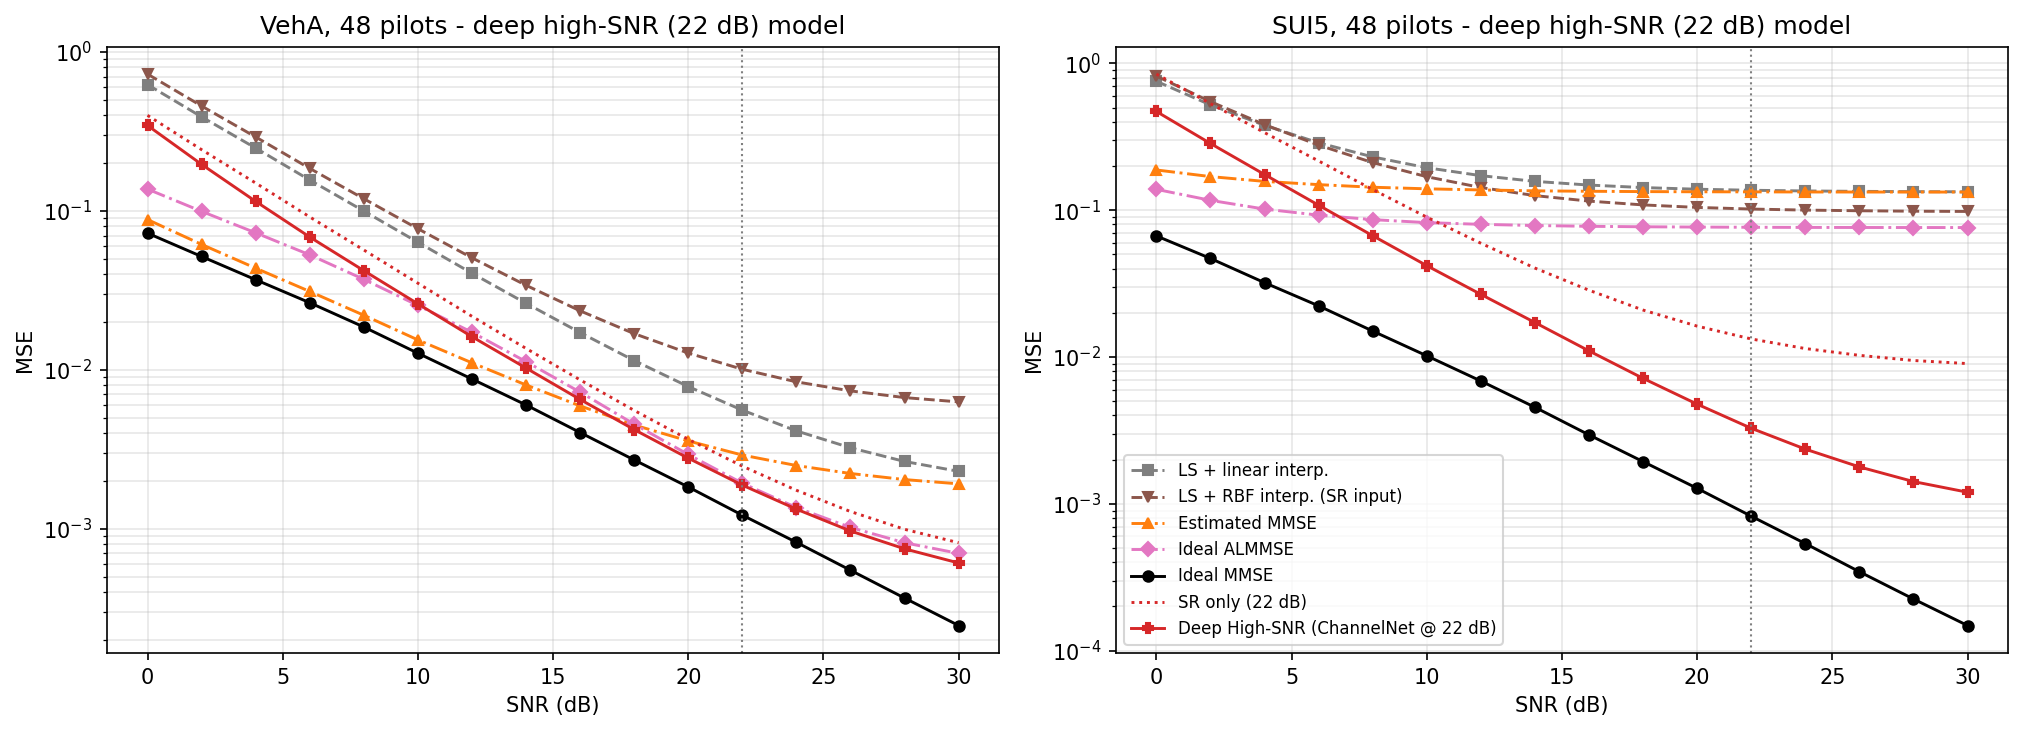
\includegraphics[width=0.86\textwidth]{Images/high_snr_VehA_vs_SUI5.png}
  \caption{Deep high-SNR (22~dB) ChannelNet against the baselines: VehA (left), SUI5 (right).}
  \label{fig:highsnr}
\end{figure}

\subsection{MSE versus number of pilots (paper Fig.~5)}

\begin{figure}[!htbp]
  \centering
  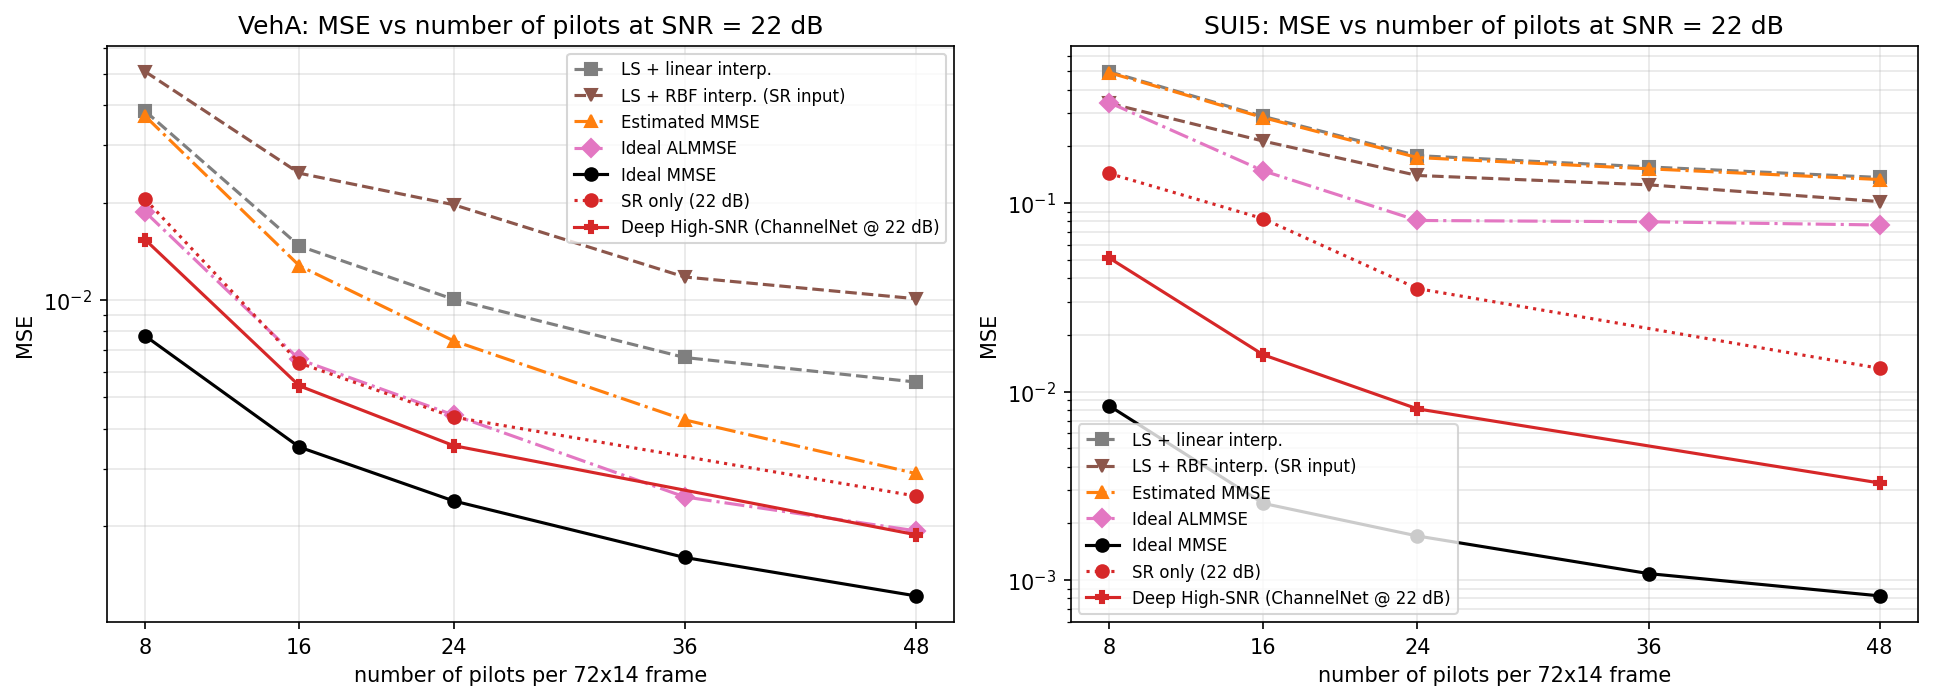
\includegraphics[width=0.86\textwidth]{Images/fig5_mse_vs_pilots_snr22.png}
  \caption{MSE vs.\ number of pilots at 22~dB (ChannelNet trained at 22~dB for each density).}
  \label{fig:pilotsweep}
\end{figure}

\begin{table}[!htbp]
  \centering
  \caption{MSE vs.\ number of pilots at 22~dB.}
  \label{tab:mse_pilots}
  \small
  \setlength{\tabcolsep}{4.5pt}
  \begin{tabular}{rcccccc}
    \toprule
    \# pilots & LS-lin & Est. MMSE & Ideal ALMMSE & Ideal MMSE & SR-22 & CN-22 \\
    \midrule
    \multicolumn{7}{l}{\textit{VehA}} \\
    48 & 5.58e-3 & 2.91e-3 & 1.94e-3 & 1.22e-3 & 2.48e-3 & \textbf{1.88e-3} \\
    24 & 1.00e-2 & 7.48e-3 & 4.41e-3 & 2.40e-3 & 4.35e-3 & \textbf{3.55e-3} \\
    16 & 1.47e-2 & 1.28e-2 & 6.55e-3 & 3.51e-3 & 6.39e-3 & \textbf{5.43e-3} \\
    8 & 3.83e-2 & 3.69e-2 & 1.87e-2 & 7.74e-3 & 2.04e-2 & \textbf{1.53e-2} \\
    \midrule
    \multicolumn{7}{l}{\textit{SUI5}} \\
    48 & 1.37e-1 & 1.33e-1 & 7.65e-2 & 8.23e-4 & 1.33e-2 & \textbf{3.27e-3} \\
    24 & 1.78e-1 & 1.74e-1 & 8.08e-2 & 1.71e-3 & 3.52e-2 & \textbf{8.09e-3} \\
    16 & 2.88e-1 & 2.84e-1 & 1.48e-1 & 2.55e-3 & 8.26e-2 & \textbf{1.57e-2} \\
    8 & 4.98e-1 & 4.92e-1 & 3.41e-1 & 8.40e-3 & 1.44e-1 & \textbf{5.11e-2} \\
    \bottomrule
  \end{tabular}
\end{table}

\subsection{Cross-check on Vienna-simulator channels}
\label{sec:vienna}

The six 48-pilot ChannelNets, trained only on the Python channel generator, were tested unchanged on 1\,000
frames from the Vienna 5G simulator (baselines with covariances from the Vienna training frames). Their MSE
differs from the matched-data results by at most \textbf{0.18~dB (VehA) and 0.32~dB (SUI5)} at every SNR
(e.g.\ deep high-SNR network at 22~dB: $1.94\cdot10^{-3}$ vs.\ $1.88\cdot10^{-3}$ on VehA,
$3.39\cdot10^{-3}$ vs.\ $3.27\cdot10^{-3}$ on SUI5), and the ranking of all methods is unchanged
(\texttt{results/figures/vienna\_*.png}). The networks depend on the channel statistics, not on the
simulator, so all conclusions hold for Vienna channels as used in the paper.

\subsection{Inferences}

\begin{enumerate}
  \item \textbf{VehA (Fig.~4a, paper Fig.~3).} ChannelNet is about 5~dB better than LS + linear interpolation at every SNR. The 12~dB and 22~dB networks are within 1.4~dB and 1.9~dB of the genie ideal MMSE at their training SNRs. They beat the ideal ALMMSE from 4~dB upwards and the estimated MMSE from 18~dB upwards (+1.9~dB at 22~dB). Below 12~dB our estimated MMSE (2 000-frame covariance) is 0.3--2.7~dB better, so the paper's ``comparable with the ideal MMSE'' at low SNR is reproduced only approximately. The ordering ideal MMSE $<$ ChannelNet $<$ ALMMSE / estimated MMSE $<$ LS at medium-to-high SNR matches the paper.
  \item \textbf{SUI5 (Fig.~4b, paper Fig.~4).} With the 10~$\mu$s delay spread, the frequency response varies faster than the pilot spacing can follow. Every interpolation-based linear estimator therefore saturates from about 10~dB (LS and estimated MMSE at 0.13, ideal ALMMSE at 0.077), as in the paper. ChannelNet keeps improving (3.3e-3 at 22~dB, 1.2e-3 at 30~dB): \textbf{16~dB better than the estimated MMSE and 13.7~dB better than the ideal ALMMSE at 22~dB} (Fig.~5). Only the ideal MMSE, which applies the exact 2-D covariance directly to the pilots, is better.
  \item \textbf{SNR-specific networks.} The 22~dB network overtakes the 12~dB network above \textbf{16~dB (VehA)} and \textbf{18~dB (SUI5)}, the switching threshold of the paper. Outside its region each network fails: the 12~dB VehA model levels off at about 3e-3 (worse than LS at 28--30~dB), and the 22~dB model is 6.8~dB above the ideal MMSE at 0~dB.
  \item \textbf{Role of the DnCNN stage.} The SR output is already 5--9~dB better than its RBF-interpolated input. The DnCNN adds 0.3--1.7~dB on VehA and \textbf{2.5--8.8~dB on SUI5}, where the SRCNN alone saturates (9e-3 at 30~dB). The two-stage cascade of the paper is essential for the harder channel.
  \item \textbf{Pilot density (Fig.~6, paper Fig.~5).} ChannelNet beats the estimated MMSE and the ideal ALMMSE at every density, as in the paper. On VehA it reaches 1.9e-3 / 3.5e-3 / 5.4e-3 / 1.5e-2 for 48 / 24 / 16 / 8 pilots, versus 2.9e-3 / 7.5e-3 / 1.3e-2 / 3.7e-2 for the estimated MMSE. The gap to the ideal MMSE grows from 1.9 to 3.0~dB. On SUI5, ChannelNet with \textbf{16 pilots is still 9~dB better than the estimated MMSE with 48 pilots}, i.e.\ it needs about a third of the pilot overhead.
  \item \textbf{Multi-SNR training.} A single network trained on 0--30~dB is within about 1~dB of the better SNR-specific network from 8 to 22~dB and beats both below 8~dB (by up to 2.5~dB). The price is up to 1.8~dB (VehA) and 4.5~dB (SUI5) at high SNR (Section 7).
\end{enumerate}

% ----------------------------------------------------------------------------
\section{Discussion: SNR-specific training and generalisation}
\label{sec:discussion}

\paragraph{Limitations.} The paper notes that the optimal weights depend on the SNR and that retraining
for every SNR is ``practically impossible because the SNR value is continuous''; it therefore uses two
networks, and its high-SNR network ``is going to fail again'' above about 23~dB. We observe the same:
\begin{enumerate}
  \item \emph{Noise-level mismatch (covariate shift).} The DnCNN learns a denoiser for one noise level;
    below its training SNR it removes too little noise (22~dB model: 6.8~dB above the ideal MMSE at 0~dB, VehA).
  \item \emph{Over-smoothing / error floor.} Above its training SNR it keeps removing ``noise'' that is
    really channel detail: the 12~dB VehA model saturates at $\approx3\cdot10^{-3}$ and is worse than plain
    LS at 28--30~dB; the 22~dB model's gap to the ideal MMSE grows from 1.9~dB (22~dB) to 3.9~dB (30~dB).
    The SR stage likewise learns an SNR-dependent, Wiener-like smoothing.
  \item \emph{Practical cost.} Several networks, an SNR estimator and a switching rule are needed, and
    SNR-estimation errors select the wrong network. The same over-specialisation applies to pilot pattern,
    Doppler and delay spread: each of the 14 networks is valid for one (channel, pattern, SNR) only.
\end{enumerate}

\paragraph{Remedies.}
\begin{enumerate}
  \item \textbf{Multi-SNR (blind) training}, as in DnCNN-B and ReEsNet --
    \emph{implemented here}: one network is within $\approx$1~dB of the better SNR-specific model from 8 to
    22~dB and beats both below 8~dB, but loses up to 1.8/4.5~dB (VehA/SUI5) at high SNR because its capacity
    is shared across noise levels.
  \item \textbf{Noise-level conditioning}: the estimated noise level as an extra input map (FFDNet)
    or as feature modulation (FiLM), so one network adapts its denoising strength continuously.
  \item \textbf{SNR bank / mixture of experts}: a few SNR-bin networks selected by an SNR estimate -- the
    strategy of the paper (switch at the 16--18~dB crossover found here).
  \item \textbf{Model-driven / unfolded networks}, e.g.\ learned denoising AMP, in which the noise
    variance enters explicitly as a parameter.
  \item \textbf{Curriculum learning and augmentation} over SNR, Doppler and delay spread;
    \textbf{untrained priors} (deep image prior), which need no training SNR at all; and
    \textbf{learned pilot design} to reduce the sensitivity to pilot density.
\end{enumerate}

\paragraph{Other limitations.} ICI (Doppler) and ISI (SUI5 delay $>$ CP) are not modelled, since the ground
truth is the channel at each symbol centre and $Y = HX + Z$. The ideal MMSE/ALMMSE use genie statistics. The
pilot study used 22~dB (the deep high-SNR operating point) instead of the 20~dB of the paper. The DnCNN
(0.67\,M parameters, $\approx$2.7~GFLOP per frame) is far costlier than a $1008\times48$ LMMSE product.

% ----------------------------------------------------------------------------
\section{Conclusion}

Treating the $72\times14$ channel grid as an image, ChannelNet reconstructs it from 48 noisy pilots by
super-resolution and denoising. On VehA it is $\approx$5~dB better than LS interpolation at every SNR,
within 1.4--1.9~dB of the genie ideal MMSE at its training SNRs and better than the estimated MMSE above
18~dB. On the long-delay SUI5 channel all practical linear estimators saturate at 0.08--0.13 while
ChannelNet keeps improving to $1.2\cdot10^{-3}$ (16~dB better than the estimated MMSE at 22~dB), as reported
in the paper. Its main weakness is SNR specificity (error floors, crossover at 16--18~dB); multi-SNR
training removes most of it with a single network, and noise-level conditioning is the natural next step.

\end{document}
